\documentclass[a0paper,portrait,fontscale=.32]{baposter}

\usepackage{wrapfig}
\usepackage{lmodern}
\usepackage{lipsum}
\usepackage[utf8]{inputenc} %unicode support
\usepackage[T1]{fontenc}

\usepackage{amsmath,amssymb,graphicx}

\usepackage{booktabs}
\usepackage{caption}
% Used for displaying a sample figure. If possible, figure files should
% be included in EPS format.
%
% If you use the hyperref package, please uncomment the following two lines
% to display URLs in blue roman font according to Springer's eBook style:
%\usepackage{color}
%\renewcommand\UrlFont{\color{blue}\rmfamily}
%
\usepackage{xcolor}

%%%%%%%%%%%%%%%%%%%%%%%%%%%%%%%%%%%%%%%%%%%%%%%%%%
% SHORTCUTS

\def\x{{\mathbf x}}
\def\L{{\cal L}}
\def\w{\mathsf{w}}

\def\C{{\mathbb C}}
\def\E{{\mathbb E}}
\def\K{{\mathbb K}}
\def\N{{\mathbb N}}
\def\P{{\mathbb P}}
\def\Q{{\mathbb Q}}
\def\R{{\mathbb R}}
\def\T{{\mathbb T}}
\def\U{{\mathbb U}}
\def\Z{{\mathbb Z}}

\def\calA{{\mathcal A}}
\def\calB{{\mathcal B}}
\def\calC{{\mathcal C}}
\def\calD{{\mathcal D}}
\def\calE{{\mathcal E}}
\def\calF{{\mathcal F}}
\def\calG{{\mathcal G}}
\def\calL{{\mathcal L}}
\def\calM{{\mathcal M}}
\def\calN{{\mathcal N}}
\def\calP{{\mathcal P}}
\def\calT{{\mathcal T}}
\def\calU{{\mathcal U}}
\def\calX{{\mathcal X}}
\def\calY{{\mathcal Y}}
\def\calZ{{\mathcal Z}}

\def\scrC{{\mathscr C}}
\def\scrS{{\mathscr S}}
\def\vv{{\mathbf v }}
\def\xx{{\mathbf x }}
\def\yy{{\mathbf y }}
\def\zz{{\mathbf z }}

\def\bzeta{{\boldsymbol \zeta}}
\def\bxi{{\boldsymbol \xi}}

\newcommand{\ep}{\varepsilon}
\newcommand{\ph}{\varphi}

\renewcommand{\Re}{\operatorname{Re}}
\renewcommand{\Im}{\operatorname{Im}}
\newcommand{\Max}{\mathop{\mathrm{Max}}}
\newcommand{\Min}{\mathop{\mathrm{Min}}}
\newcommand{\softmin}{\mathop{\mathrm{softmin}}}
\newcommand{\softmax}{\mathop{\mathrm{softmax}}}
\newcommand{\argmin}{\mathop{\mathrm{Argmin}}}
\newcommand{\argmax}{\mathop{\mathrm{Argmax}}}
\newcommand{\ds}{\displaystyle}
\renewcommand{\ker}{\mathrm{Ker}}
\newcommand{\im}{\mathrm{Im}}
\newcommand{\id}{\mathrm{Id}}
\newcommand{\Supp}{\mathrm{Supp}}
\newcommand{\sgn}{\mathrm{sgn}}
\newcommand{\indic}{\mathbf{1}}
\newcommand{\loc}{\mathrm{loc}}
\newcommand{\sinc}{\mathrm{sinc}}
\newcommand{\diag}{\operatorname{diag}}
   
\newcommand{\tv}{\mathrm{TV}}
\newcommand{\vp}{\mathrm{vp}}
\newcommand{\Pf}{\mathrm{Pf}}

\newcommand{\ii}{\Gamma}


\newcommand{\Var}{\mathrm{Var}}
\newcommand{\Cov}{\mathrm{Cov}}

\newcommand{\kl}{\operatorname{KL}}
\newcommand{\js}{D_{\text{JS}}}

\newcommand{\vertiii}[1]{{\left\vert\kern-0.25ex\left\vert\kern-0.25ex\left\vert #1 
    \right\vert\kern-0.25ex\right\vert\kern-0.25ex\right\vert}}

\newcommand{\gmm}{\mathsf{GMM}}
\newcommand{\rmd}{\mathrm{d}}
\newcommand{\rmP}{\mathrm{P}}
\newcommand{\NN}{\mathcal{N}}

\usepackage{pifont}
\newcommand{\cmark}{{\color{green!50!black}\ding{51}~}}%
\newcommand{\xmark}{{\color{red}\ding{55}~}}%

\renewcommand{\arraystretch}{1.0}

% --------- tweak these once ----------
\newcommand{\imgW}{0.15\linewidth}
\newcommand{\cropW}{0.15\linewidth}
\newcommand{\lab}[1]{\scriptsize\textsf{#1}}
\newcommand{\CROPID}{crop000}
\newcommand{\SIGID}{sigma7.00}
\newcommand{\IMGDIR}{figs/synth} 


%\DeclareMathOperator*{\argmax}{arg\,max}
%\DeclareMathOperator*{\argmin}{arg\,min}

% \usepackage{hyperref}
% \usepackage{url}
% \usepackage{amsthm}
% \usepackage{diagbox}
% \usepackage{multirow}
% \usepackage{tablefootnote}
% \usepackage{algorithm2e}
% \usepackage{arydshln}
% \usepackage{multirow, makecell}
% \usepackage{tikz}
% \usepackage{subcaption,wrapfig}
% \usepackage{lipsum}
% \usepackage[most]{tcolorbox}
% \usepackage{ulem}
% %\usepackage{appendixnumberbeamer}
% \usepackage{booktabs,array}

% \usepackage{float}

% \usepackage{pifont}
% \newcommand{\cmark}{{\color{green!50!black}\ding{51}~}}%
% \newcommand{\xmark}{{\color{red}\ding{55}~}}%
% \RestyleAlgo{ruled}
% \usetikzlibrary{spy}
% \usepackage{booktabs,array}
% \usepackage{amsfonts}
% \def\Midrule{\midrule[\heavyrulewidth]}
% \newcount\rowc
% \usepackage[export]{adjustbox}
% %\usepackage{unicode-math}
% %\usepackage{cmbright}
% % Optional math commands from https://github.com/goodfeli/dlbook_notation.

% \RestyleAlgo{ruled}
% \usetikzlibrary{spy}
% %
% \usepackage{booktabs,array}
% \usepackage{amsfonts}
% \def\Midrule{\midrule[\heavyrulewidth]}
% \newcount\rowc

% \usepackage{amsmath}

% \newcommand{\new}{\marginpar{NEW}}
% \newcommand{\norm}[1]{||{#1}||}
% \newcommand{\prox}{\operatorname{Prox}}
% \newcommand{\rprox}{\operatorname{Rprox}}
% \newcommand{\id}{\operatorname{Id}}
% \newcommand{\dom}{\operatorname{dom}}
% \renewcommand{\Im}{\operatorname{Im}}
\newtheorem{assumption}{Assumption}
\newtheorem{remark}{Remark}
\newtheorem{thm}{Theorem}
\newtheorem{cor}{Corollary}
\newtheorem{proposition}{Proposition}
\newtheorem{definition}{Definition}
% \newcommand{\noise}{\xi}
% \newcommand{\dime}{n}
% \newcommand{\bfit}[1]{\textbf{\textit{#1}}}
% \usepackage{tikz}
% \usetikzlibrary{arrows.meta}
% \usetikzlibrary{positioning}
% \usetikzlibrary{calc}

% \selectcolormodel{cmyk}

% \graphicspath{{figures/}} % Directory in which figures are stored

% \newcommand{\compresslist}{%
% \setlength{\itemsep}{0pt}%
% \setlength{\parskip}{1pt}%
% \setlength{\parsep}{0pt}%
% }

% \newenvironment{boenumerate}
%   {\begin{enumerate}\renewcommand\labelenumi{\textbf\theenumi.}}
%   {\end{enumerate}}

% \newcommand{\xdownarrow}[1]{%
%   {\left\Downarrow\vbox to #1{}\right.\kern-\nulldelimiterspace}
% }

\newcommand{\mycite}[1]{{\color{cyan}[{#1}]}}
\newcommand{\best}[1]{\textbf{#1}}
\newcommand{\second}[1]{\underline{#1}}

\begin{document}


\definecolor{darkindigo}{RGB}{75, 0, 130}
\definecolor{darkblue}{RGB}{0,0,139}

\begin{poster}
{
grid=false,
headerborder=open, 
colspacing=1em, 
bgColorOne=white,
bgColorTwo=white,
borderColor=black!45,
headerColorOne=darkblue, %!55!black,
headerColorTwo=darkindigo, %!75!black,
headerFontColor=white,
boxColorOne=white,
textborder=rounded,
eyecatcher=false,
headerheight=0.13\textheight,
headershape=rounded,
headershade=plain,
headerfont=\Large\textsf,
linewidth=2pt
}
{}
%
%----------------------------------------------------------------------------------------
%	TITLE AND AUTHOR NAME
%----------------------------------------------------------------------------------------
%
{
\textsf %Sans Serif
{
{ \hspace*{-1cm} Controllable Blind Deblurring \\ with Diffusion Models } \\
}
} % Poster title
% {\vspace{0.2em} Add Author Name, Add another author name\\ 
% {\small \vspace{0.7em} Department of Computing, TU Dublin, Tallaght, Dublin, Ireland}} 
{\sf\vspace{0.2em}
I. Si Salah$^{1,2}$, E. Cribelier$^{1}$, T. Veit$^{1}$, W. Hauser$^{1}$, A. Leclaire$^{2}$
\\[0.2em]
\small{$^{1}$ DxO Labs} \quad \small{$^{2}$ LTCI, Télécom Paris, IP Paris} \\
\small{
  isisalah@dxo.com % Author email addresses
}
}
{

\includegraphics[height=.08\linewidth]{figs/DxO_Labs_logo.png}
\hspace{1cm}
\includegraphics[height=.13\linewidth]{figs/logo_telecom_paris_ipp.png}}

% this states the box starts at column 0 (edge of page), row 0 (top of page) for a span of 3 (columns wide)
%ù\headerbox{Introduction}{name=introduction,column=0,row=0, span=3}{ Place an over view of your research - use your executive summary or abstract as a pointer of what information to place in here.
%\vspace{2cm} %remove this, only added for spacing
%}

% this states the box starts at column 0 (edge of page), directly below the box labelled introduction for a span of 1 (column wide)


\headerbox{1) Blind Deblurring Problem}{name=blind_deblur,column=0,span=1}{

\textsc{Main goal:} perform blind image sharpening for real-world photographs with very high resolution.
\medskip

$\bullet$ \textbf{Blur sources:}
  \begin{itemize}
    \item[$\cdot$] \textit{Physical}: lens softness/defocus, camera shake/ motion.
    \item[$\cdot$] \textit{Processing}: over-aggressive denoising.
  \end{itemize}

$\bullet$ \textbf{Blind deblurring} is ill-posed: both the sharp image and the blur kernel are unknown. \\

$\bullet$ Recovering details requires \textbf{plausible generation}.\\

$\bullet$ Need for explicit \textbf{control over restoration strength}.\\

$\rightarrow$ \textsc{Solution}: \textbf{controllable blind deblurring} with \textbf{stable diffusion (SD) generative prior}.

}
\headerbox{2) Latent Diffusion Models (LDM)}{name=diffusion,column=0,span=1,below=blind_deblur}{

  $\bullet$ \textbf{Latent diffusion:} encode image $\xx_0$ to latent
  \[\zz_0=E(\xx_0) , \]
  run the following diffusion in latent space, then decode
  \[\hat{\xx}_0=D(\zz_0) . \]

$\bullet$ \textbf{Forward process:} for a noise schedule ${\beta_t\in(0,1)}$,
  $\alpha_t=1-\beta_t$, $\bar{\alpha}_t=\prod_{s=1}^t \alpha_s$, forward sampling consists in
  % \[
  %   q(\zz_t \mid \zz_0)=\mathcal{N}\!\left(\sqrt{\bar{\alpha}_t}\,\zz_0,\ (1-\bar{\alpha}_t)I\right)
  % \]
  \[
    %  \quad \Leftrightarrow \quad
    \zz_t=\sqrt{\bar{\alpha}_t}\,\zz_0+\sqrt{1-\bar{\alpha}_t}\,\boldsymbol{\epsilon},\ 
    \boldsymbol{\epsilon}\sim\mathcal{N}(0,I).
  \]

$\bullet$ \textbf{Backward process:} sample $z_T \sim \mathcal{N}(0,I)$ and then
  \[
    \zz_{t-1}=
    \frac{1}{\sqrt{\alpha_t}}
    \left(\zz_t-\frac{\beta_t}{\sqrt{1-\bar{\alpha}_t}}\,\epsilon_\theta(\zz_t,t)\right)
    +\sigma_t\boldsymbol{\eta},
  \]
  with $\boldsymbol{\eta}\sim\mathcal{N}(0,I)$, and where $\epsilon_\theta(\zz_t,t)$ is a neural network that is trained to predict the noise in $\zz_t$. \\

$\bullet$ \textbf{Training loss:}
  \[
    \mathcal{L}(\theta)=
    \mathbb{E}_{t,\zz_0,\boldsymbol{\epsilon}}
    \left[\left\|\boldsymbol{\epsilon}-\epsilon_\theta(\zz_t,t)\right\|_2^2\right].
  \]
}

\headerbox{3) Proposed Approach: Latent Diffusion Model Conditioning}{name=dm_conditioning,column=1,span=2}{
  \begin{center}
    \textbf{Training}
    
  \begin{minipage}{.45\linewidth} \centering
      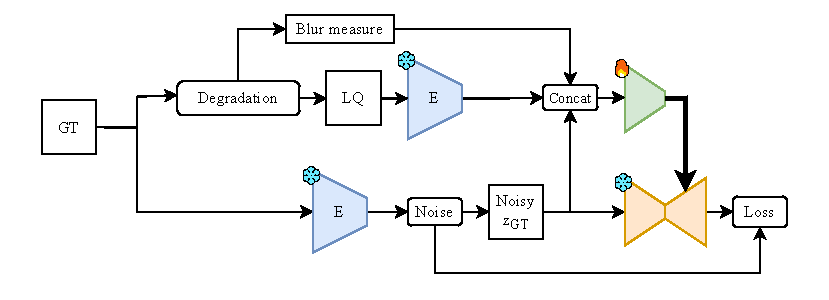
\includegraphics[width=.95\linewidth]{figs/cldm_train-Page-1.drawio.png}\par
      \vspace{0.2em}
      {\small \textbf{ControlNet style conditioning (CN)} \\ SD UNet is frozen}\par
   \end{minipage}
   \begin{minipage}{.54\linewidth} \centering
     \vskip 3mm
     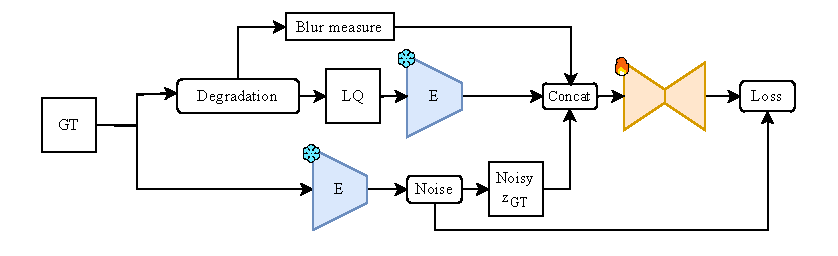
\includegraphics[width=.95\linewidth]{figs/ldm_train-Page-1.drawio.png}\par
     \vspace{0.2em}
     {\small \textbf{Direct LDM finetuning conditioning (FT)} \\ SD UNet is finetuned}\par
   \end{minipage}
   \bigskip
   
   In both cases, training is done with the loss: \hspace{2mm}
   $
     \calL(\theta)
     = \mathbb{E}_{t,\,\zz_0,\,\boldsymbol{\epsilon}_t} 
     \left[ \,\big\|\boldsymbol{\epsilon}_t - \boldsymbol{\epsilon}_\theta(\zz_t, t,\zz_{LQ},\mathsf{BM})\big\|_2^2 \,\right] .
   $
     
  \medskip
  \rule{.25\linewidth}{0.4pt}
  \vspace{0.1em}

  \begin{minipage}{.53\linewidth} \centering
    \textbf{Super-Sharpen (SupS) \\ with LDM conditional inference} \\
    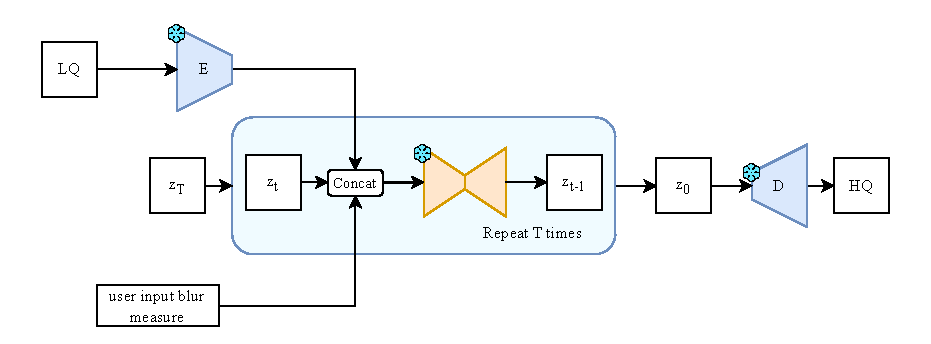
\includegraphics[width=\linewidth]{figs/ldm_sample-Page-2.drawio.png} \\
  \end{minipage}
  \begin{minipage}{.46\linewidth}
  %   \begin{center}
  %     \textbf{Controllable Blind Deblurring} \\[0.1em]
  %     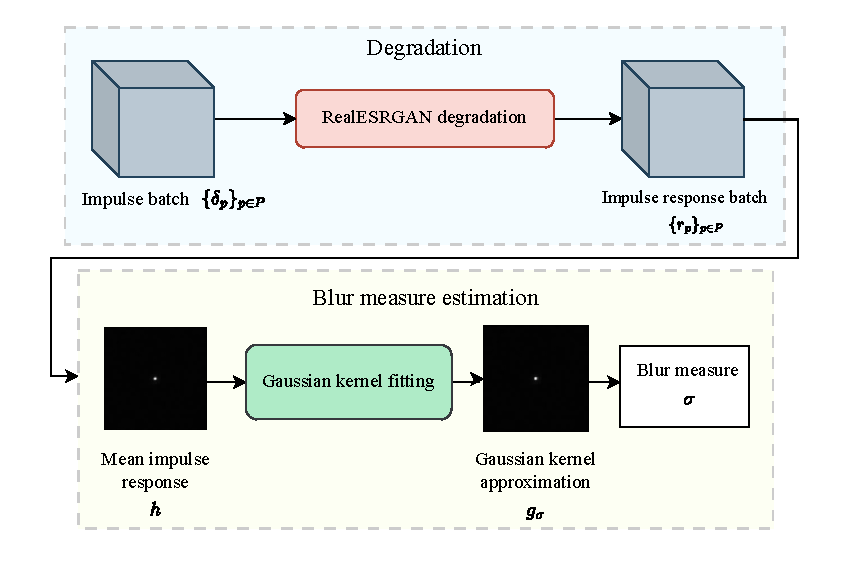
\includegraphics[width=\linewidth]{figs/BxU_diagram.drawio.png}
  %   \end{center}[-0.9em]
  %   \small
  %   $\cdot$ Explicit control of the fidelity/innovation trade-off. \\
    % $\cdot$ Blur measure is the std of the estimated Gaussian blur kernel.
  \centering
  \vskip 2mm
  \textbf{Controllable Blind Deblurring}\\
  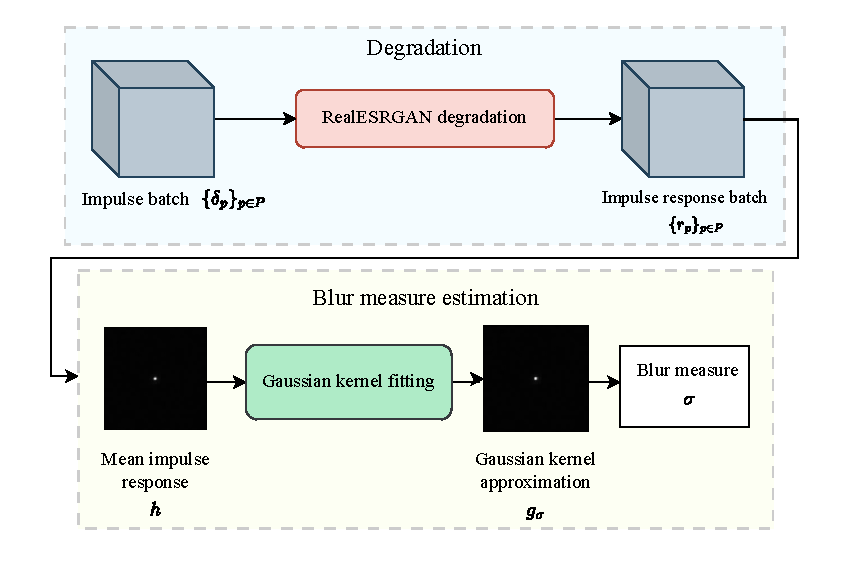
\includegraphics[width=.85\linewidth]{figs/BxU_diagram.drawio.png}\\[-0.9em] 
  \scriptsize
  Blur measure (BM): std of the estimated Gaussian blur kernel
  \end{minipage}
 
  
\end{center}

}


\headerbox{4) Synthetic Results}{name=results_synth,column=1,span=2,below=dm_conditioning}{

\centering


\scalebox{1}{%
\begin{tabular}{lrrrrrr}
\toprule
& \multicolumn{3}{c}{Full-reference} & \multicolumn{3}{c}{No-reference} \\
\cmidrule(lr){2-4}\cmidrule(lr){5-7}
Method & PSNR $\uparrow$ & SSIM $\uparrow$ & LPIPS $\downarrow$ & MUSIQ $\uparrow$ & MANIQA $\uparrow$ & CLIP-IQA $\uparrow$ \\
\midrule
DiffBIR [3]        & 18.3051 & 0.5284 & 0.2278 & \second{71.6563} & 0.5986 & \second{0.7107} \\
PASD [4]           & \best{21.9344} & \best{0.6518} & 0.2138 & 68.9798 & 0.4850 & 0.5904 \\
SeeSR [5]          & 20.1731 & 0.5808 & 0.2463 & 70.4701 & 0.5529 & 0.6541 \\
ResShift [6]       & 19.7569 & 0.4976 & 0.4138 & 48.0120 & 0.2960 & 0.4199 \\
\midrule
SupS-CN  & 19.7659 & 0.5549 & \second{0.2020} & \best{71.7406} & \best{0.6493} & \best{0.7299} \\
SupS-FT  & \second{20.7670} & \second{0.6138} & \best{0.1714} & 71.0819 & \second{0.6112} & 0.7102 \\
\bottomrule
\end{tabular}%
}

\vspace{0.3em}
{\best{Best} bold, \second{second-best} underlined.}

\vspace{0.5em}

\scalebox{0.7}{%
\begin{tabular}{@{}cccccccc@{}}
{\small LQ} & {\small DiffBIR [3]} & {\small PASD [4]} & {\small SeeSR [5]} & {\small ResShift [6]} & {\small SupS-CN} & {\small SupS-FT} & {\small HQ} \\[0.1em]
{\small PSNR$\uparrow$/ LPIPS$\downarrow$} & {\small 19.45/0.20} & {\small 22.77/0.26} & {\small 20.06/0.40} & {\small 21.08/0.71} & {\small 18.88/0.27} & {\small 20.28/0.18} & {\small --} \\
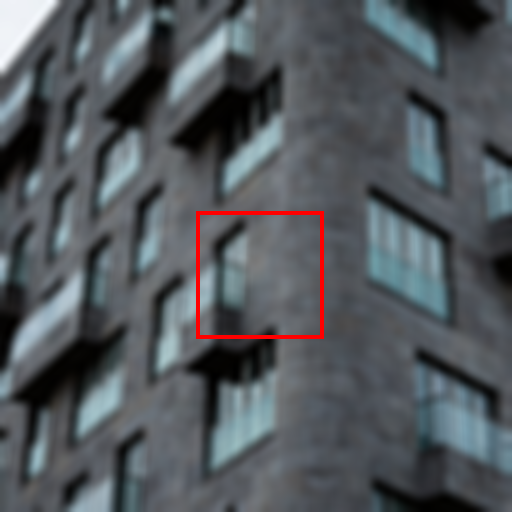
\includegraphics[width=\imgW]{figs/synth/img_001_crop000_sigma7.00_lq_boxed.png} &
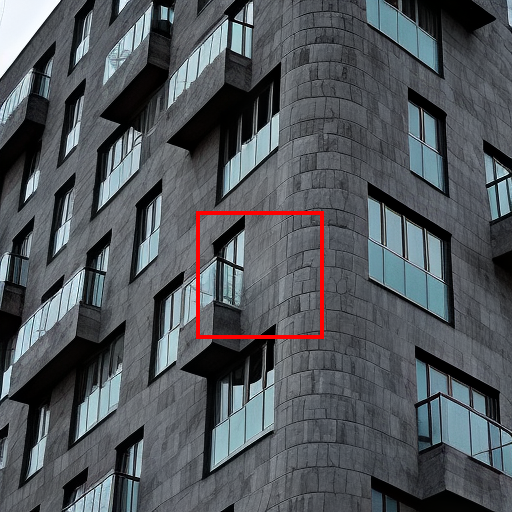
\includegraphics[width=\imgW]{figs/synth/img_001_crop000_sigma7.00_diffbir_boxed.png} &
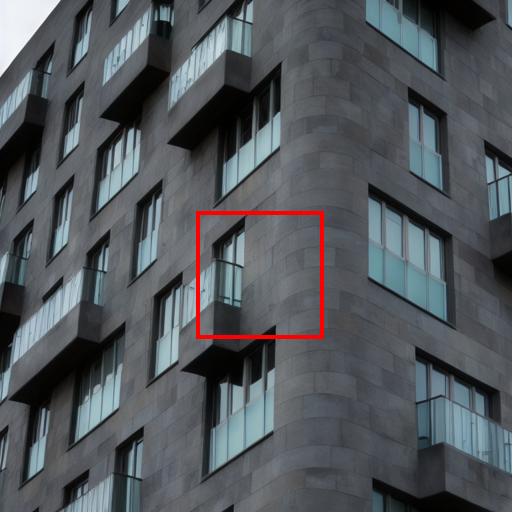
\includegraphics[width=\imgW]{figs/synth/img_001_crop000_sigma7.00_pasd_boxed.png} &
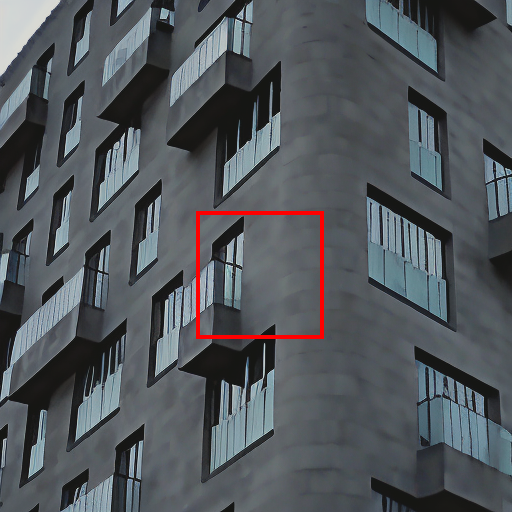
\includegraphics[width=\imgW]{figs/synth/img_001_crop000_sigma7.00_seesr_boxed.png} &
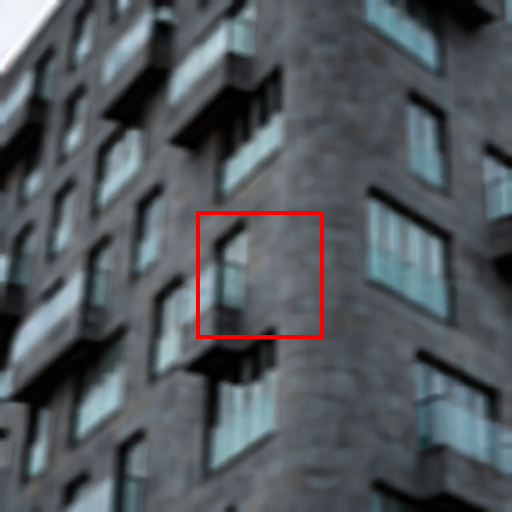
\includegraphics[width=\imgW]{figs/synth/img_001_crop000_sigma7.00_resshift_boxed.png} &
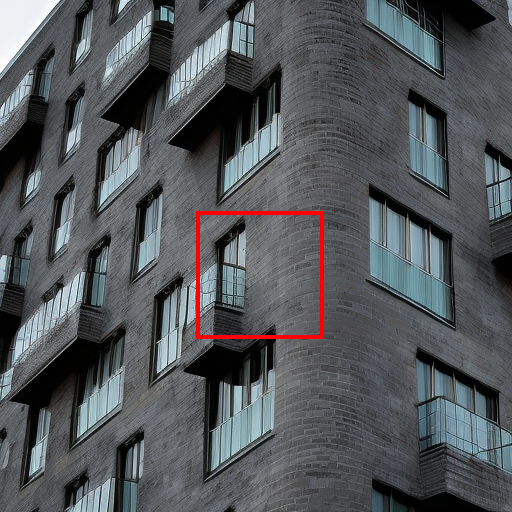
\includegraphics[width=\imgW]{figs/synth/img_001_crop000_sigma7.00_s1.0_bxu7.00_cldm_boxed.png} &
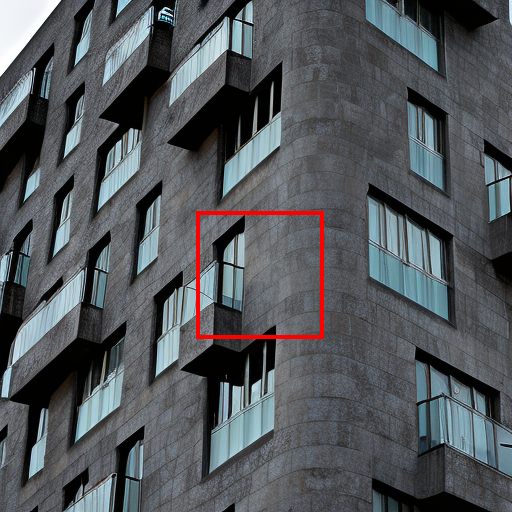
\includegraphics[width=\imgW]{figs/synth/img_001_crop000_sigma7.00_s1.0_bxu7.00_ldm_boxed.png} &
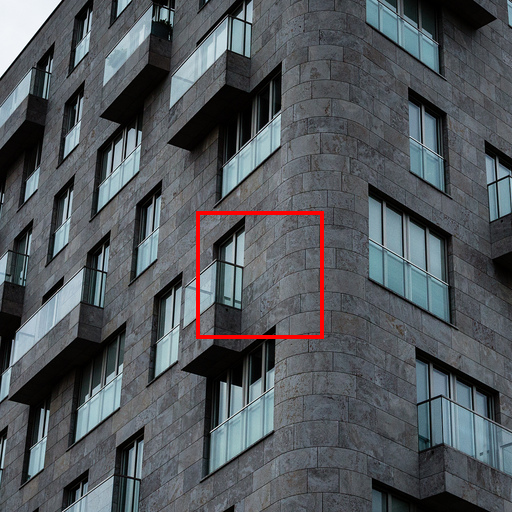
\includegraphics[width=\imgW]{figs/synth/img_001_crop000_hq_boxed.png} \\

\includegraphics[width=\cropW]{figs/synth/img_001_crop000_sigma7.00_lq_crop.png} &
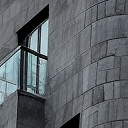
\includegraphics[width=\cropW]{figs/synth/img_001_crop000_sigma7.00_diffbir_crop.png} &
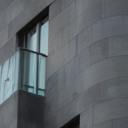
\includegraphics[width=\cropW]{figs/synth/img_001_crop000_sigma7.00_pasd_crop.png} &
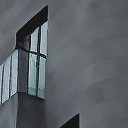
\includegraphics[width=\cropW]{figs/synth/img_001_crop000_sigma7.00_seesr_crop.png} &
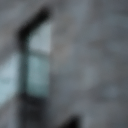
\includegraphics[width=\cropW]{figs/synth/img_001_crop000_sigma7.00_resshift_crop.png} &
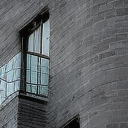
\includegraphics[width=\cropW]{figs/synth/img_001_crop000_sigma7.00_s1.0_bxu7.00_cldm_crop.png} &
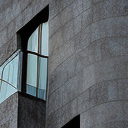
\includegraphics[width=\cropW]{figs/synth/img_001_crop000_sigma7.00_s1.0_bxu7.00_ldm_crop.png} &
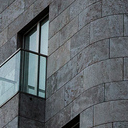
\includegraphics[width=\cropW]{figs/synth/img_001_crop000_hq_crop.png} \\[0.1em]
{\small PSNR$\uparrow$/ LPIPS$\downarrow$} & {\small 19.13/0.08} & {\small 22.14/0.13} & {\small 20.50/0.14} & {\small 19.06/0.46} & {\small 18.03/0.13} & {\small 20.09/0.07} & {\small --} \\
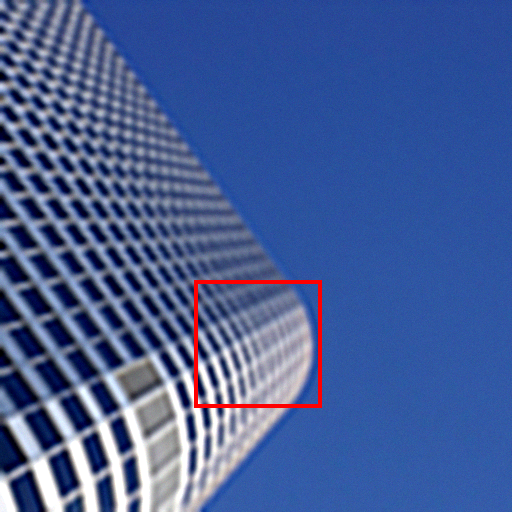
\includegraphics[width=\imgW]{figs/synth/img_005_crop001_sigma4.63_lq_boxed.png} &
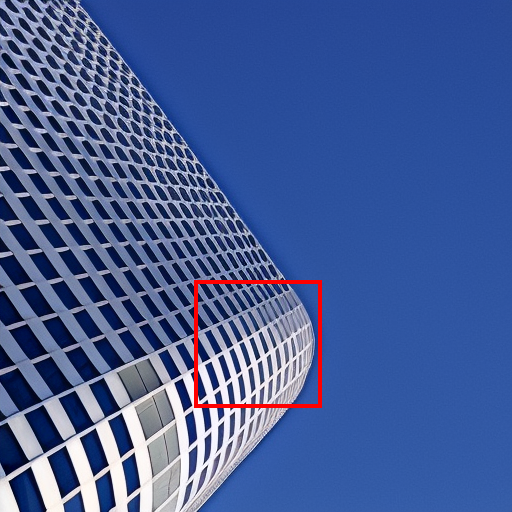
\includegraphics[width=\imgW]{figs/synth/img_005_crop001_sigma4.63_diffbir_boxed.png} &
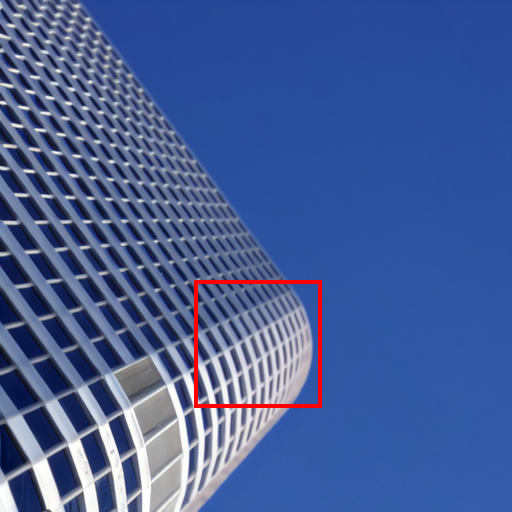
\includegraphics[width=\imgW]{figs/synth/img_005_crop001_sigma4.63_pasd_boxed.png} &
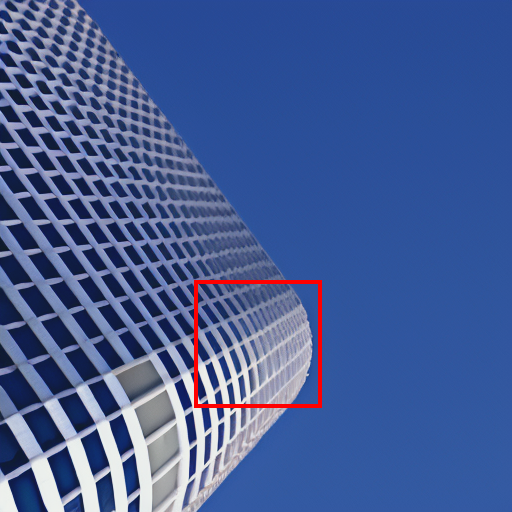
\includegraphics[width=\imgW]{figs/synth/img_005_crop001_sigma4.63_seesr_boxed.png} &
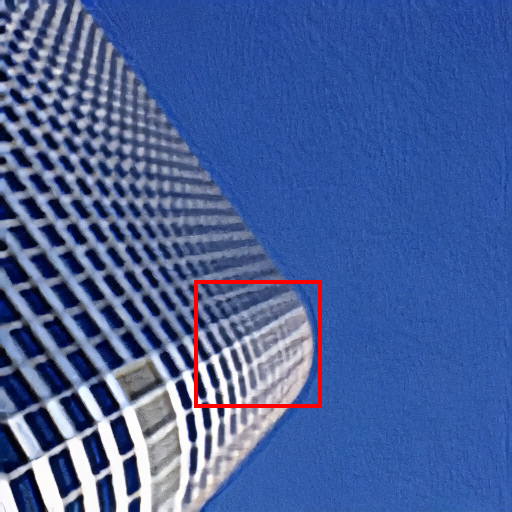
\includegraphics[width=\imgW]{figs/synth/img_005_crop001_sigma4.63_resshift_boxed.png} &
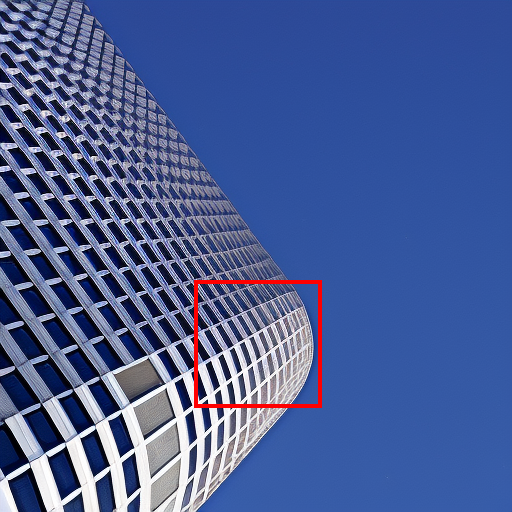
\includegraphics[width=\imgW]{figs/synth/img_005_crop001_sigma4.63_s1.0_bxu4.63_cldm_boxed.png} &
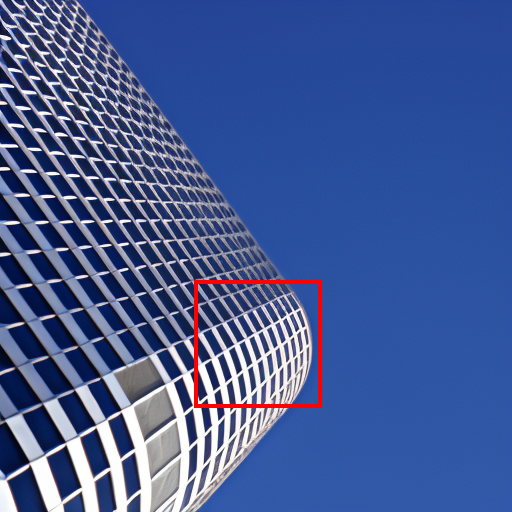
\includegraphics[width=\imgW]{figs/synth/img_005_crop001_sigma4.63_s1.0_bxu4.63_ldm_boxed.png} &
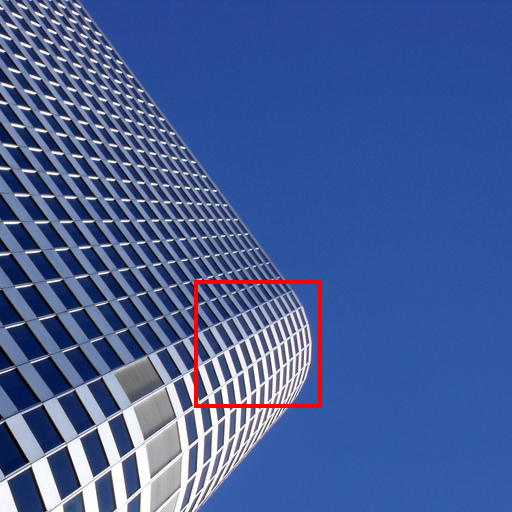
\includegraphics[width=\imgW]{figs/synth/img_005_crop001_hq_boxed.png} \\

\includegraphics[width=\cropW]{figs/synth/img_005_crop001_sigma4.63_lq_crop.png} &
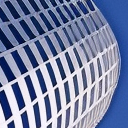
\includegraphics[width=\cropW]{figs/synth/img_005_crop001_sigma4.63_diffbir_crop.png} &
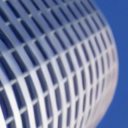
\includegraphics[width=\cropW]{figs/synth/img_005_crop001_sigma4.63_pasd_crop.png} &
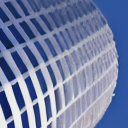
\includegraphics[width=\cropW]{figs/synth/img_005_crop001_sigma4.63_seesr_crop.png} &
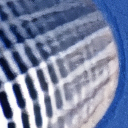
\includegraphics[width=\cropW]{figs/synth/img_005_crop001_sigma4.63_resshift_crop.png} &
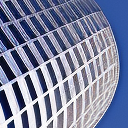
\includegraphics[width=\cropW]{figs/synth/img_005_crop001_sigma4.63_s1.0_bxu4.63_cldm_crop.png} &
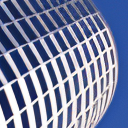
\includegraphics[width=\cropW]{figs/synth/img_005_crop001_sigma4.63_s1.0_bxu4.63_ldm_crop.png} &
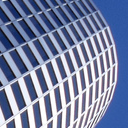
\includegraphics[width=\cropW]{figs/synth/img_005_crop001_hq_crop.png} \\

\end{tabular}%
}


}

\headerbox{5) Real-world Result with SupS-FT}{name=results_real,column=1,span=2,below=results_synth}{ 

\centering

\begin{tabular}{cccc} 
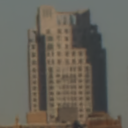
\includegraphics[width=.22\columnwidth]{figs/real/a0071-kme_490_cr_cr.png} &
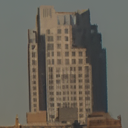
\includegraphics[width=.22\columnwidth]{figs/real/a0071-kme_490_cr_cr_s2_bxu0.70_ldms.png} &
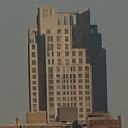
\includegraphics[width=.22\columnwidth]{figs/real/a0071-kme_490_cr_cr_s2_bxu3.00_ldms.png} &
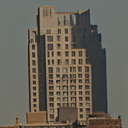
\includegraphics[width=.22\columnwidth]{figs/real/a0071-kme_490_cr_cr_s2_bxu8.00_ldms.png} \\
{\small LQ} & {\small BM = 0.7} & {\small BM = 3.0} & {\small BM = 8.0}
\end{tabular}


}

\headerbox{6) Conclusion}{name=conclusion,column=0,span=1,below=diffusion}{
  $\bullet$ We propose a controllable blind deblurring method based on diffusion models. \\
  $\bullet$ We study two conditioning strategies: \textbf{ControlNet-style} and \textbf{direct LDM fine-tuning}. \\
  $\bullet$ SupS-CN performs better w.r.t. no-reference metrics but is biased by the frozen SD backbone. \\
  $\bullet$ SupS-FT approach achieves better perceptual similarity (LPIPS) and is generally more faithful to the blurry input.

 \textsc{Future work}: Better enforce data consistency and force identity-behavior when the blur measure is zero. Explore newer generative backbones.
  
}

\headerbox{References}{name=references,column=0,span=1,below=conclusion}{
  \footnotesize
  % Latent Diffusion
  [1] R. Rombach et al. %A. Blattmann, D. Lorenz, P. Esser, \& B. Ommer
  High-resolution image synthesis with latent diffusion models.
  CVPR, 2022. % the IEEE/CVF conference on computer vision and pattern recognition (pp. 10684-10695). \\

  % DDPM
  % $\cdot$ J. Ho, A. Jain, \& P. Abbeel. Denoising diffusion probabilistic models.
  % NeurIPS 2020.\\

  % ControlNet
  [2] L. Zhang et al. % A. Rao, \& M. Agrawala
  Adding conditional control to text-to-image diffusion models.
  ICCV, 2023. % the IEEE/CVF international conference on computer vision (pp. 3836-3847).

  % DiffBIR
  [3] Lin et al. %, X., He, J., Chen, Z., Lyu, Z., Dai, B., Yu, F., ... & Dong, C. 
  DiffBIR: Toward blind image restoration with generative diffusion prior.
  ECCV, 2024.
  % (pp. 430-448). Cham: Springer Nature Switzerland.

  % PASD
  [4] T. Yang et al. % , R. Wu, P. Ren, X. Xie, and L. Zhang,
  Pixel-aware stable diffusion for realistic image SR and personalized stylization.
  ECCV, 2024.

  % SeeSR
  [5] R. Wu et al. % , T. Yang, L. Sun, Z. Zhang, S. Li, and L. Zhang,
  SeeSR: Towards semantics-aware real-world image super-resolution.
  CVPR, 2024.

  % ResShift
  [6] Z. Yue et al. %, J. Wang, and C. C. Loy,
  ResShift: Efficient diffusion model for image super-resolution by residual shifting.
  NeurIPS, 2023.

  % Real-ESRGAN
  [7] X. Wang et al.
  Real-ESRGAN: Training real-world blind super-resolution with pure synthetic data.
  ICCV, 2021.
}
\end{poster}

\end{document}
